\subsection{Déroulement de la mission}

Pour mener à bien ce projet, nous avons décidé de suivre le calendrier suivant :
\begin{itemize}
    \item 1 semaine de recherche documentaire
    \item 3 semaines de développement de POC et de rédaction de rapport pour Panorama 
    \item 1 semaine de restitution à l'équipe de Panorama et de soutenance
\end{itemize}


\subsubsection*{Recherche Documentaire}
\addcontentsline{toc}{subsubsection}{Recherche Documentaire}

La première semaine de notre projet Activ'ESAIP nous a permis de nous familiariser avec le projet. Après une matinée de présentation de la mission par l'équipe de Panorama Performance, nous avons décidé de nous répartir les concepts importants qu'il nous fallait maîtriser pour sa réalisation, à savoir : 
\begin{itemize}
    \item M. \textsc{Girou} s'est occupé des recherches sur le concept de \textbf{Séquenceur}
    \item M. \textsc{Barbault} s'est chargé du \textbf{Lean Manufacturing}
    \item M. \textsc{Carrillo} a concentré ses recherches sur le \textbf{Management Visuel}
\end{itemize}

À la suite de cette semaine de recherches, nous avons chacun présenté le fruit de nos recherche et en avons ressorti des questions sur les points qui nous semblaient flous, de manière à pouvoir les poser à Mme. \textsc{Oudard} lors de la réunion que nous avions planifié le $1^{er}$ avril.\\

Nous avons également ressorti de cette première semaine le support le plus adapté pour garder l'aspect interactif de la solution, qui repose beaucoup sur le toucher. Notre première idée était de proposer un écran tactile de grande envergure, mais ce support s'avère très onéreux, donc peu accessible pour des PME et TPE. Nous avons donc arrêté notre choix sur un vidéo projecteur interactif comme ceux disponibles à l'ESAIP. 

\subsubsection*{Développement de la POC}
\addcontentsline{toc}{subsubsection}{Développement de la POC}

\begin{figure}[!h]
    \centering
    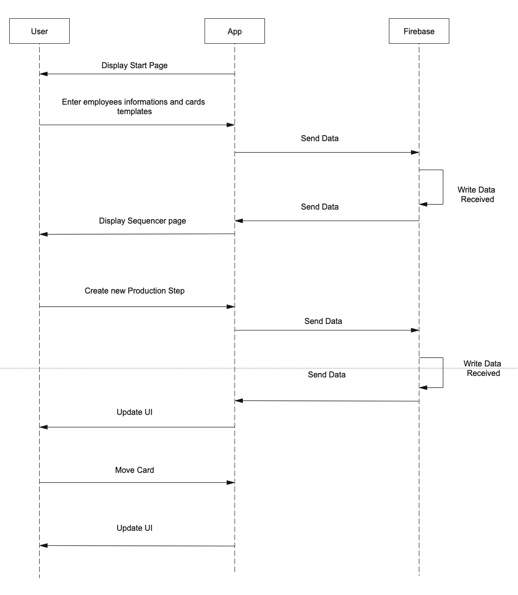
\includegraphics[scale=1]{img/sequence.jpeg}
    \caption{Le diagramme de séquence de l'application}
    \label{fig:POC}
\end{figure}


Durant les 3 sprints, respectivement du 19 au 23 avril, du 17 au 21 mai et du 31 mai au 4 juin, nous avons consacré nos efforts sur le développement d'une POC fonctionnelle.\\

Lors de la première semaine de développement, nous avons réussi à présenter à Panorama Performance une première version avec un tableau à double entrée présentant les deadlines de produit ainsi qu'un calendrier. Les “item\_production" (cf. figure \ref{fig:appV1}) pouvaient être stockés sur la base de données Firebase et l'application était déjà scrollable\footnote{Comprendre par ici que l'on peut faire défiler les lignes et colonnes à l'aide de la souris} selon les deux axes.\\


\clearpage


\begin{figure}[!h]
    \centering
    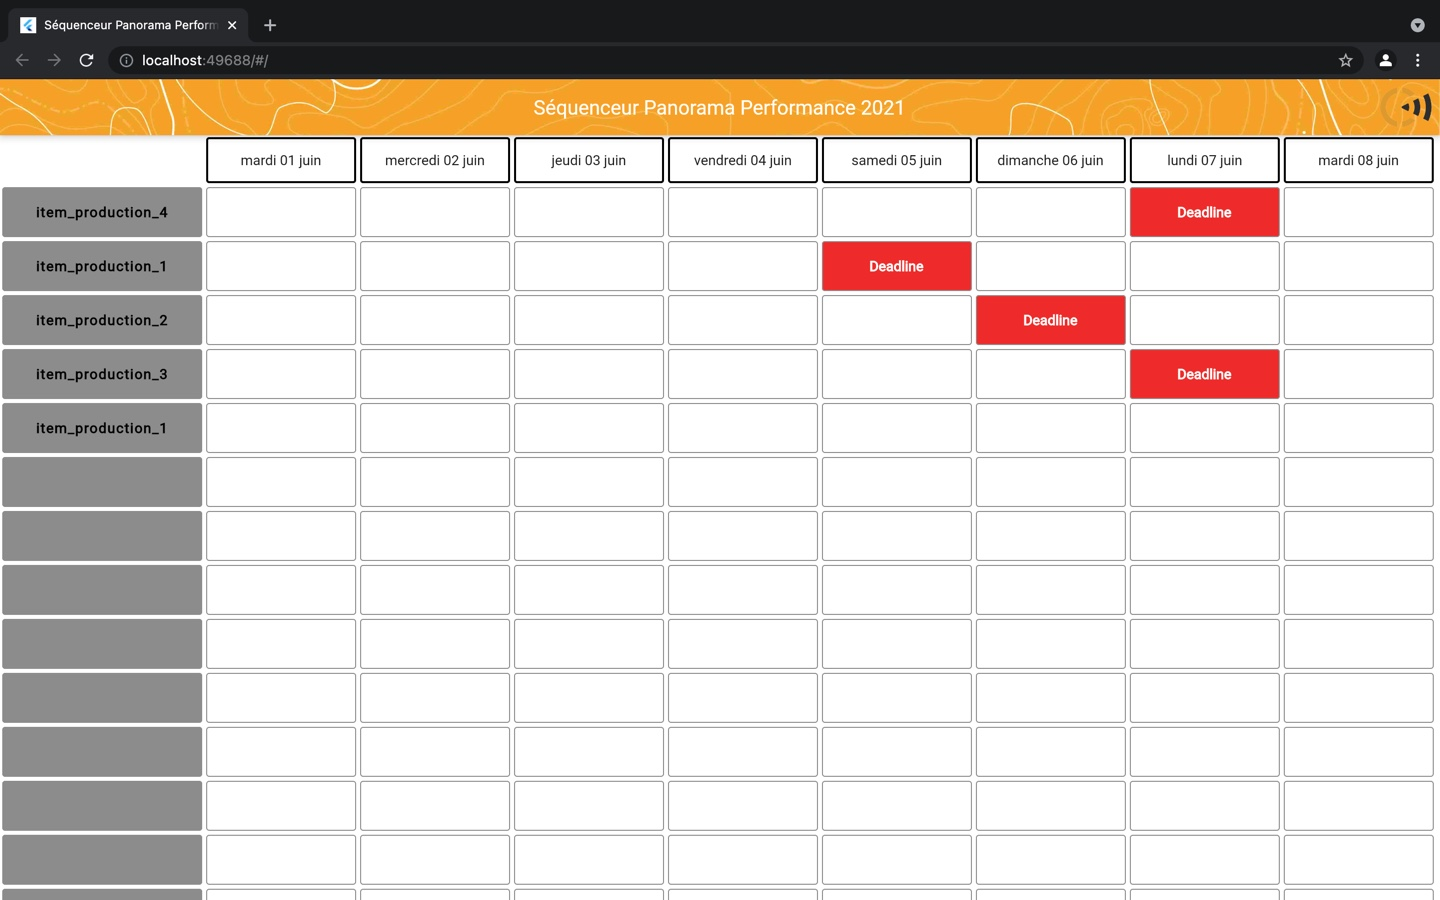
\includegraphics[scale=0.28]{img/app_v1.jpeg}
    \caption{Visuel de l'application après une semaine de développement}
    \label{fig:appV1}
\end{figure}

Nous avons également eu le temps de réaliser une page d'accueil qui permet à la fois la création de modèles pour les cartes (qui serviront à remplir la grille plus tard), ainsi que celle des différents salariés de l'entreprise et la tâche à laquelle ils peuvent être assignés. La page d'accueil est également munie de validators qui vérifient les différentes valeurs fournies par l'utilisateur avant de les écrire dans la base de données\footnote{Visible en rouge sur la figure \ref{fig:appV1StartPage}}.

\begin{figure}[!h]
    \centering
    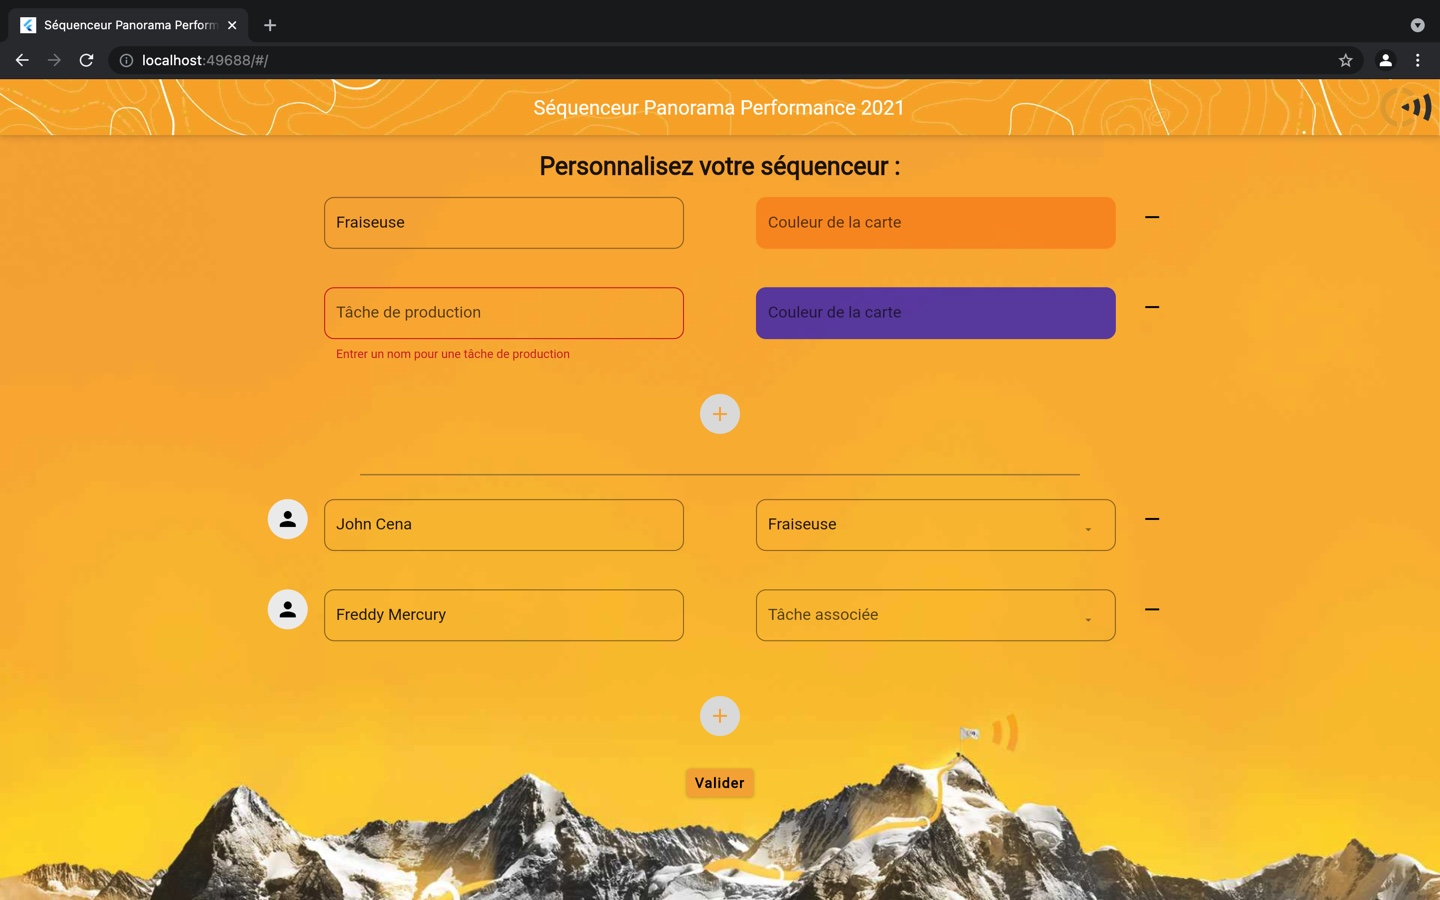
\includegraphics[scale=0.28]{img/app_v1_startPage.jpeg}
    \caption{La page d'accueil de l'application}
    \label{fig:appV1StartPage}
\end{figure}
\clearpage

L'objectif de la deuxième semaine a été de permettre la création d'étapes de production et de les récupérer pour les afficher dans la ligne qui leur correspondait.\\

Nous avons eu quelques difficultés à récupérer toutes les étapes correspondantes à une ligne de production, en effet comme vous pouvez le voir sur la figure \ref{fig:appV2}, les lignes possédant plusieurs étapes affichaient des erreurs. Cependant, la version que nous avons rendue à la fin de sprint offrait tout de même la possibilité de créer de nouvelles étapes de productions en tapotant sur une case vide d'une ligne munie d'un item de production. 


\begin{figure}[!h]
    \centering
    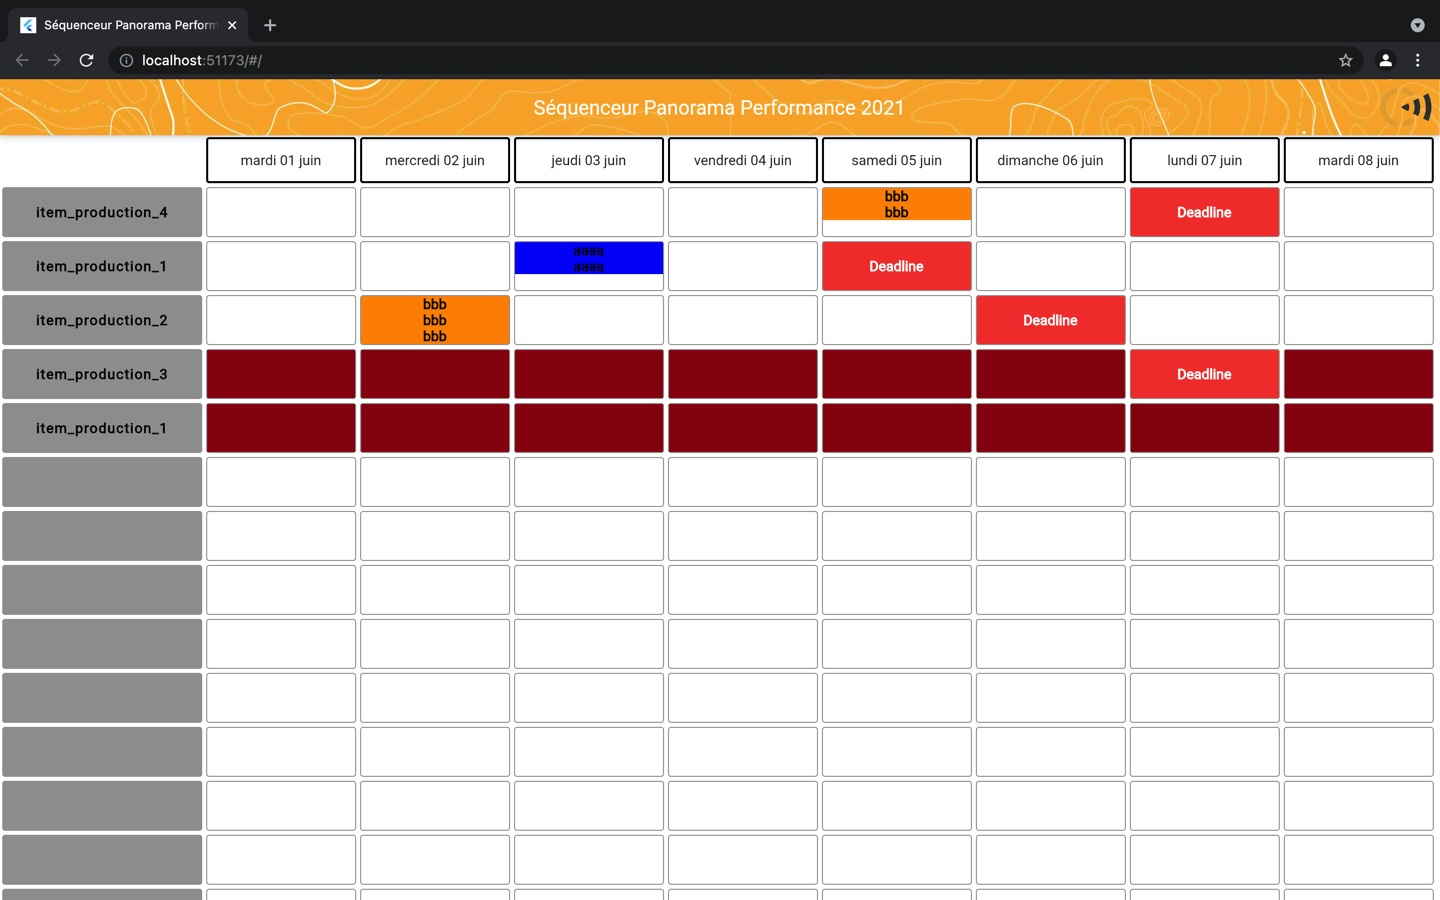
\includegraphics[scale=0.28]{img/app_v2.jpeg}
    \caption{Visuel de l'application à la fin du deuxième sprint}
    \label{fig:appV2}
\end{figure}

\begin{figure}[!h]
    \centering
    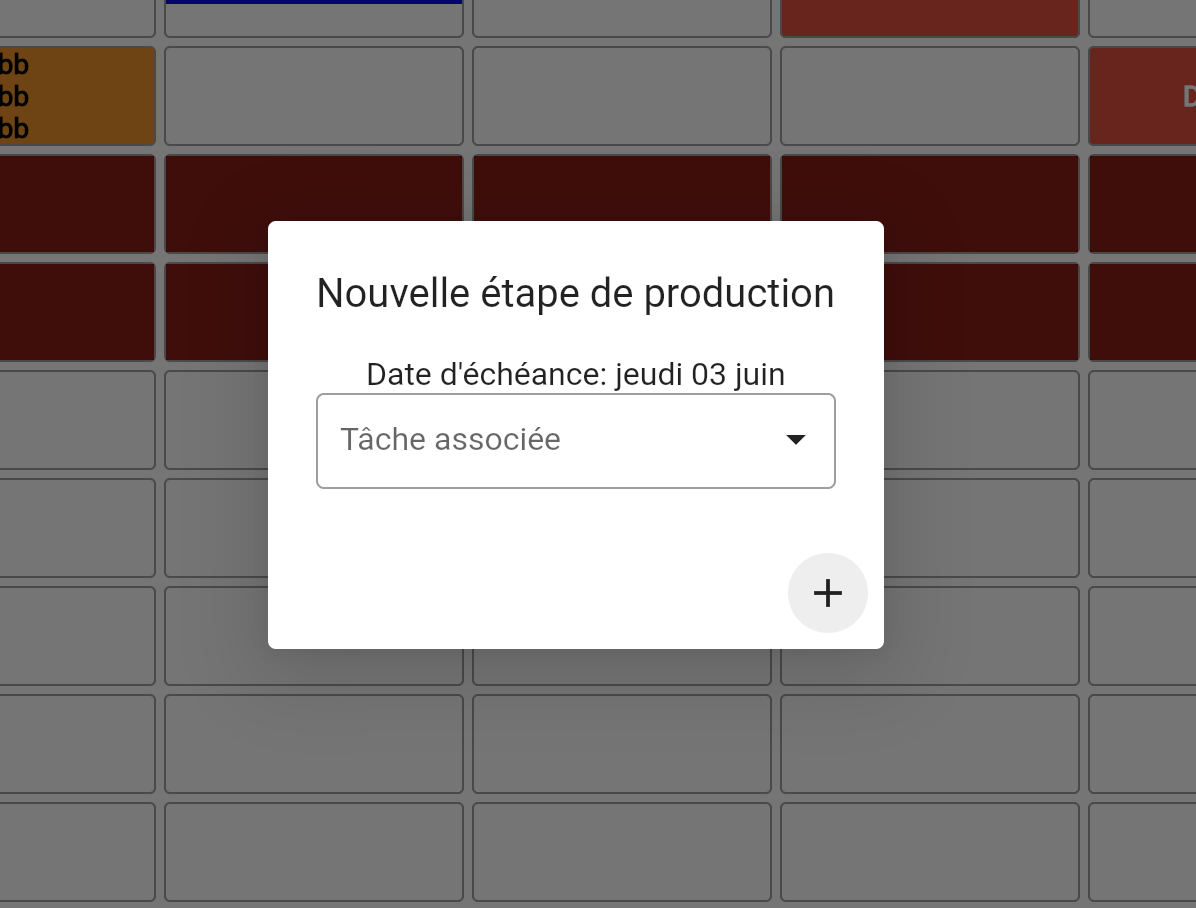
\includegraphics[scale=0.28]{img/creation_step.png}
    \caption{Fenêtre de création d'étape de production}
    \label{fig:creationStep}
\end{figure}

Nous avons également créé le formulaire de création d'items de production \footnote{correspondant à une ligne} et d'étapes de production \footnote{correspondant à une case} (voir figure \ref{fig:creationStep}). qui offre la possibilité de choisir une compétence parmi celles entrées dans la page de personnalisation du séquenceur (voir figure \ref{fig:appV1StartPage}). Les étapes apparaissent ensuite de la couleur choisie dans la ligne qui leur correspond.
\clearpage

Nous avions conclu avec Panorama Performance que la POC serait prête pour la fin du $3^{e}$ sprint, mais pour coller avec leurs disponibilités, nous avons dû avancer la date au mercredi 2 juin. Ainsi, la version que nous leur avons présentée n'était pas exempte de bugs, mais elle était belle et bien fonctionnelle.


\begin{figure}[!h]
    \centering
    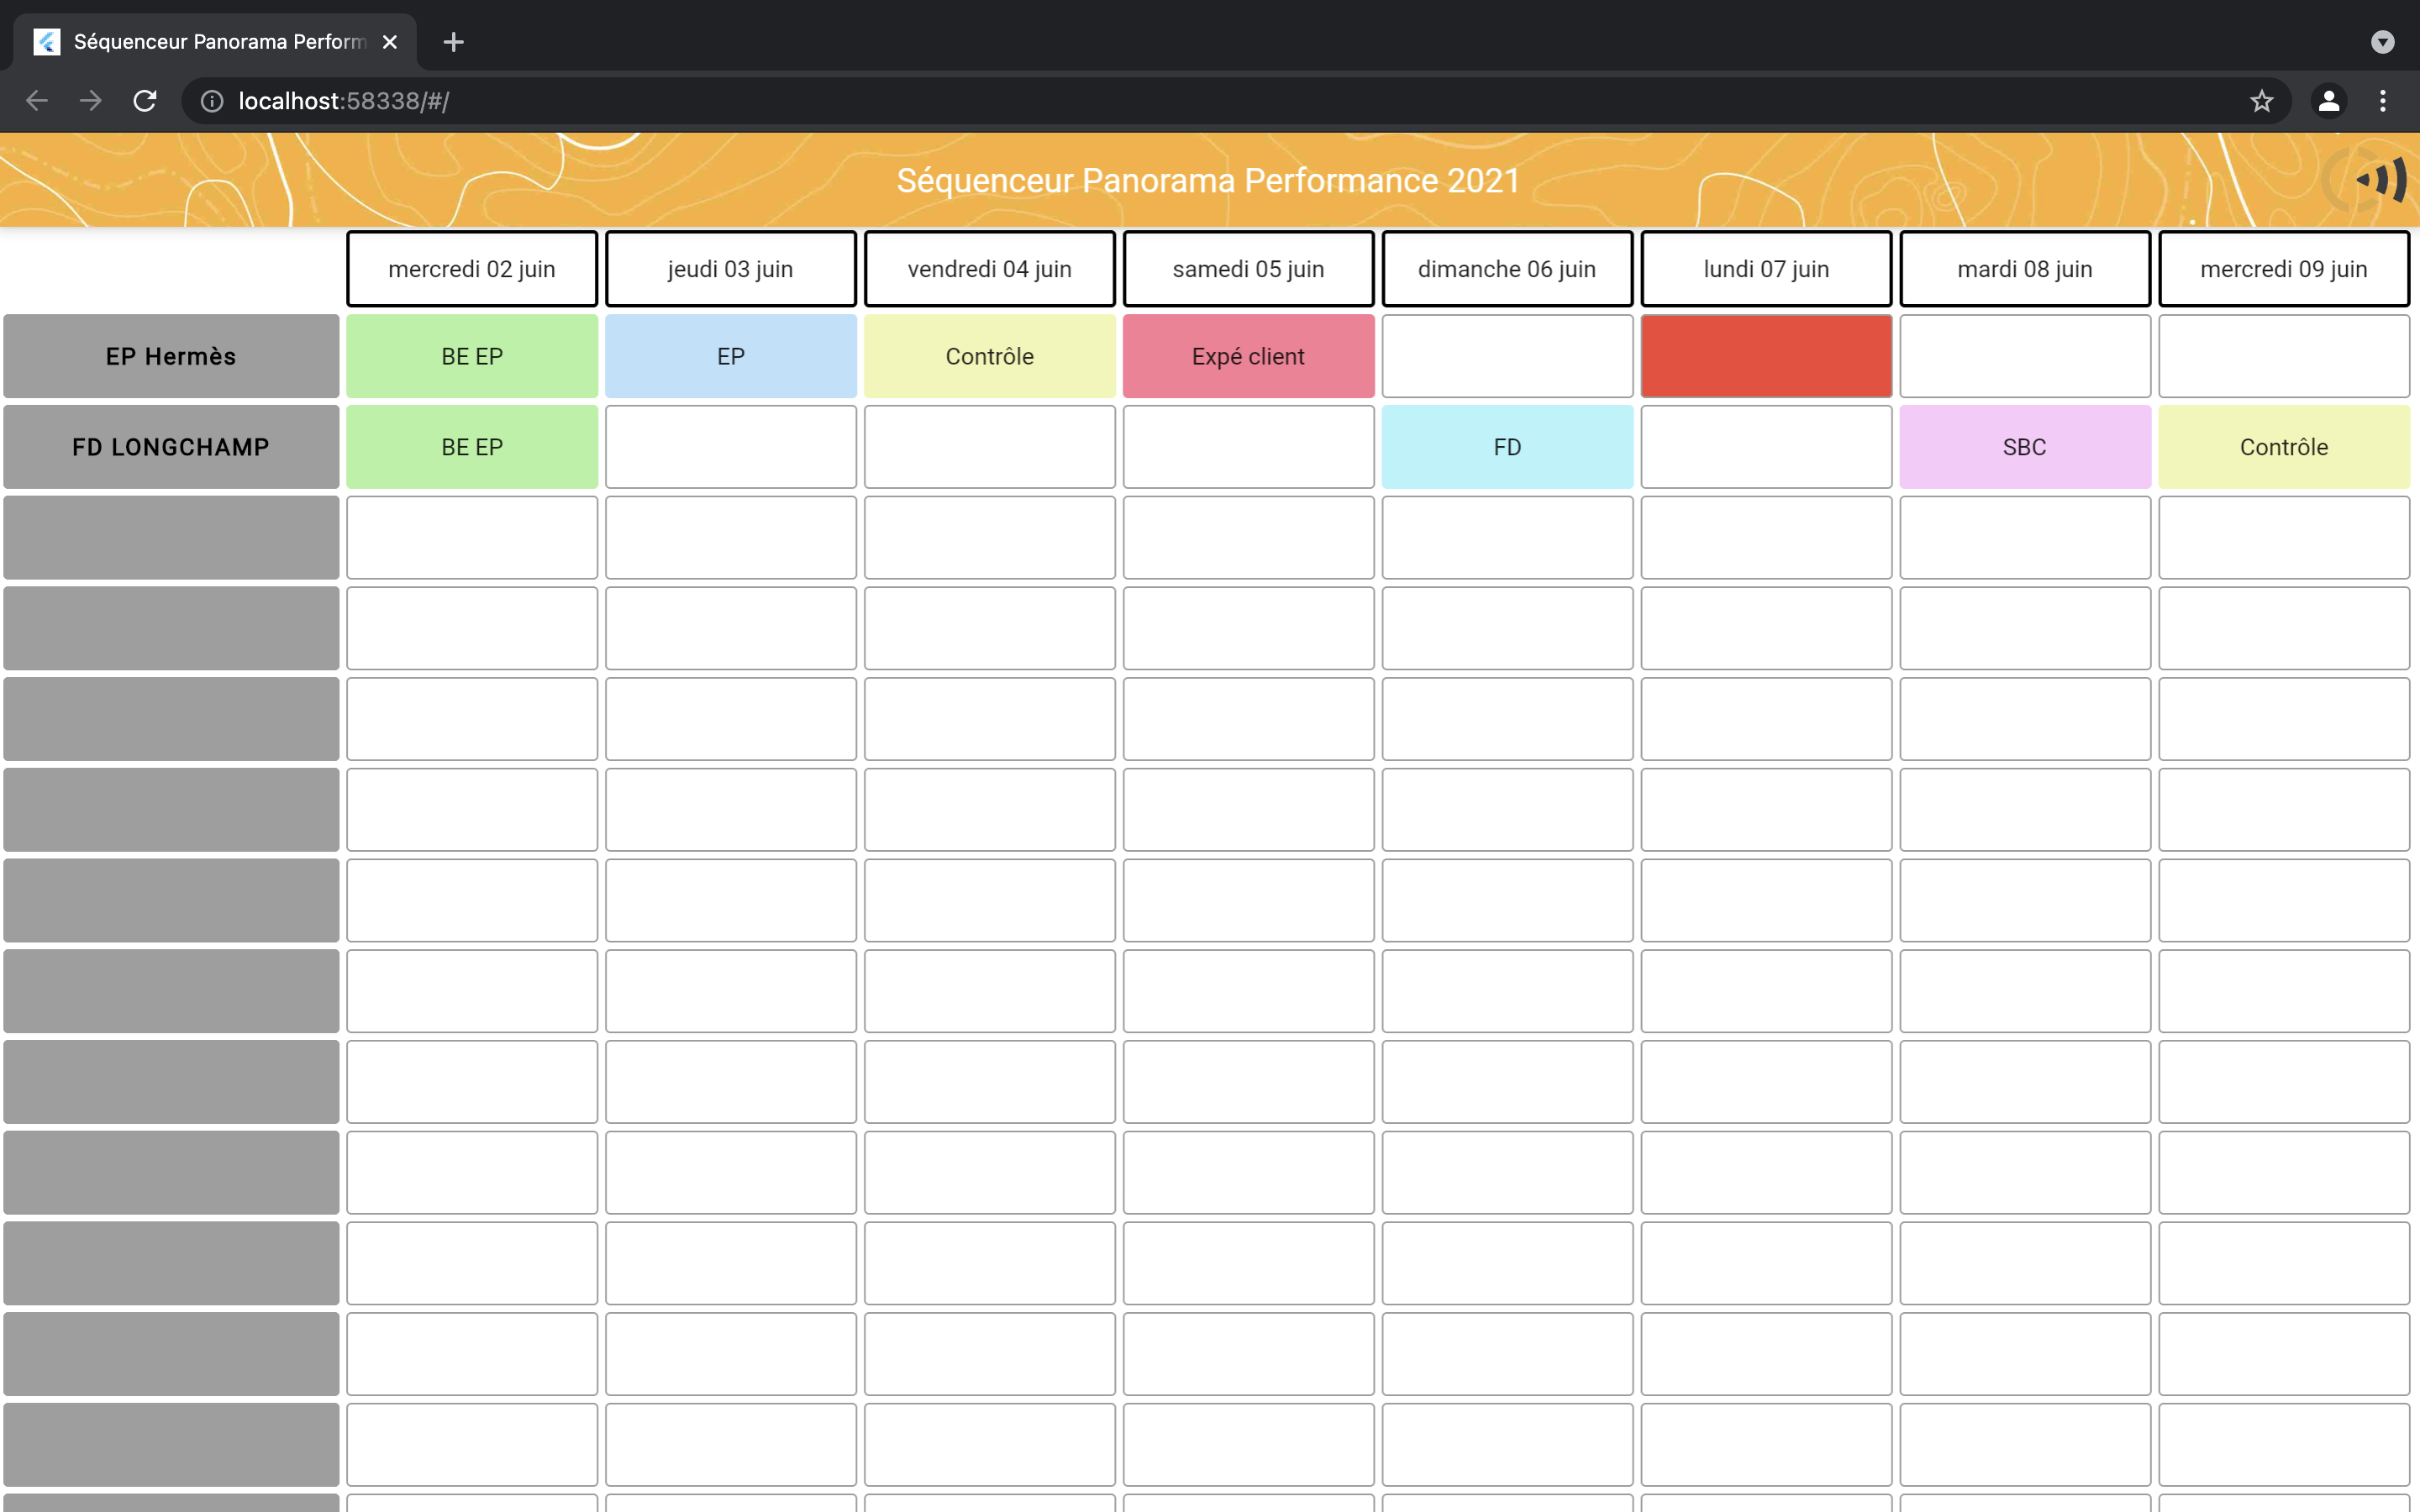
\includegraphics[scale=0.28]{img/app_v3.png}
    \caption{Visuel de la POC telle qu'est sera rendue à Panorama Performance}
    \label{fig:POC}
\end{figure}


Comme vous pouvez le voir ci-dessus, dans la figure \ref{fig:POC}, la POC est une version plus complète que les versions précédentes. Nous avons eu le temps d'y ajouter le déplacement des cartes d'étapes de production. Cela offre la possibilité de ré-arranger leur ordre ou changer leur date d'exécution.\\
\hfill

La $3^{e}$ semaine de développement à également été l'occasion de présenter notre POC à l'équipe de Panorama Performance. Nous voulions leur présenter une application fonctionnelle pour qu'ils aient la possibilité de l'essayer en s'appuyant sur un cas réel. L'essai s'est très bien déroulé et M. \textsc{Lecointre} et Mme. \textsc{Oudard} se sont avérés agréablement surpris par la facilité d'utilisation de l'application.\\

Le test s'étant déroulé dans la salle \textbf{E004} de l'ESAIP, nous avons eu la chance pouvoir utiliser le \textbf{VPI} pour présenter l'application dans un contexte réel d'utilisation. L'application s'est avérée très simple à utiliser avec les stylos “tactiles" du VPI, et la taille d'écran a parue satisfaisante pour remplacer la solution actuelle. La manière dont nous avons désigné la création et le déplacement de carte a aussi plu à Panorama Performance : plus contraignante que la version papier, elle obligerait ainsi les entreprises à utiliser les flux tirés\footnote{Certaines méthodologies des flux tirés sont peu naturelles à mettre en place (ne pas faire tourner les machines en permanence à plein régime, se plier au rythme du poste le plus lent, \dots )}




\subsubsection*{Rédaction du rapport de faisabilité}
\addcontentsline{toc}{subsubsection}{Rédaction du rapport de faisabilité}


\todo{À faire par Valentin ??}

